% !TEX encoding = UTF-8
% !TEX TS-program = pdflatex
% !TEX root = ../tesi.tex

%**************************************************************
\chapter{Descrizione dello stage}
\label{cap:descrizione-stage}
%**************************************************************

\intro{In questo capitolo verrà descritto in dettaglio l'idea dello stage, l'azienda dove è stato svolto e come è stato organizzato il lavoro.}

%**************************************************************

\section{L'azienda}

Sync Lab S.r.l. è un'azienda di consulenza informatica nata nel 2002 nella sede di Napoli e trasformatasi molto velocemente nel corso degli anni in System Integrator grazie ad un processo di maturazione delle competenze tecnologiche. Supporta le esigenze di innovazione dei clienti offrendo soluzioni IT in ambito Business Consultancy, Project Financing e IT Consultancy.
\begin{figure}[h]
	\begin{center}
		
\includegraphics[width=7cm]{logo_large}
		\caption{Logo di Sync Lab}
	\end{center}
\end{figure}
Ad oggi l'azienda conta un organico di circa 200 dipendenti ed è riuscita a coprire tutto il territorio nazionale fino ad ottenere un totale di cinque sedi a Roma, Napoli, Verona, Padova e Milano.\\
L'azienda, propone sul mercato prodotti software, attraverso essi Sync Lab ha gradualmente conquistato significativamente fette di mercato nei seguenti settori: mobile, videosorveglianza e sicurezza delle infrastrutture informatiche aziendali.
Il loro obiettivo é quello di supportare il cliente nella Realizzazione, Messa in Opera e Governance di soluzioni IT, sia dal punto di vista Tecnologico, sia nel Governo del Cambiamento Organizzativo.

%**************************************************************
\section{L'idea dello stage}

Il progetto da svolgere proposto dall'azienda per lo stage è una web application chiamata NFTLab legata all'ambito blockchain e NFT, due argomenti che stanno spopolando al momento e rendono contemporanea ed interessante il progetto di stage.\\
In dettaglio quando l'utente accede al sito potrà visualizzare le opere multimediali in vendita, fare l'accesso o la registrazione al sito. Dopo essere acceduto, l'utente potrà caricare le proprie opere e decidere se metterle in vendita o meno. Inoltre potrà sfogliare il catalogo delle opere presenti e decidere di comprarne a sua volta.\\
Essendo legato al concetto di blockchain e NFT le azioni di compravendita verranno effettuate tramite lo scambio di una moneta virtuale detta Ethereum. Un utente nel momento in cui carica un'opera diventa l'autore ed il proprietario di quest'ultima, ma se la venderà l'acquirente diventerà il nuovo proprietario ma solo l'utente che ha caricato l'opera è e sarà sempre l'autore.\\
Per realizzare questi aspetti sono state implementate diverse maschere, ovvero interfacce utente, tramite il framework Vue.js, uno strumento utile allo sviluppo di web application.\\
Parte del percorso di stage è stata riservata ad un periodo di studio (senza implementazioni se non a scopo didattico) delle tecnologie legate al back end , in particolare il framework Spring.

%**************************************************************
\section{Organizzazione del lavoro}

\subsection{Modello di sviluppo}

L'azienda adotta il modello di sviluppo Agile che si basa sull'interazione continua con gli stakeholder e predilige:
\begin{itemize}
	\item gli individui e le loro interazioni piuttosto che i processi e gli strumenti;
	\item il software funzionante piuttosto che una documentazione esaustiva;
	\item la collaborazione con il cliente piuttosto che la negoziazione dei contratti;
	\item essere propositivi verso il cambiamento piuttosto che rifiutarlo.
\end{itemize}
L'idea di questo modello non si basa quindi su uno sviluppo sequenziale ma sul concetto di rivedere di continuo le specifiche adeguandole durante l'avanzamento dello sviluppo software. In questo modo si possono apportare agilmente modifiche mediante metodologie iterative ed incrementali ed un continuo scambio di pareri ed informazioni tra gli sviluppatori ed il committente. Il progetto di stage è stato portato avanti utilizzando il metodo Scrum.\\
Scrum è il metodo più diffuso e prevede di dividere il progetto in blocchi di lavoro detti sprint, alla fine dei quali si crea un incremento del prodotto software. Esso prevede vari meeting per controllare il lavoro svolto ed organizzare il lavoro da svolgere nel prossimo periodo. Inoltre nel corso dello sviluppo l'azienda organizza diversi meeting con gli stakeholder e i membri del progetto per valutare l'andamento dello sprint.\\
Gli incontri legati a questo modello di sviluppo che vengono svolti di solito sono:
\begin{itemize}
	\item sprint planning meeting: tenuto ad inizio sprint per poter organizzare il lavoro;
	\item daily scrum: riunione giornaliera del team di sviluppo per monitorare l'andamento dello sprint;
	\item sprint review: tenuto a fine sprint per valutare i risultati ottenuti e quali cambiamenti apportare per lo sprint successivo.
\end{itemize}
\begin{figure}[h]
	\begin{center}
		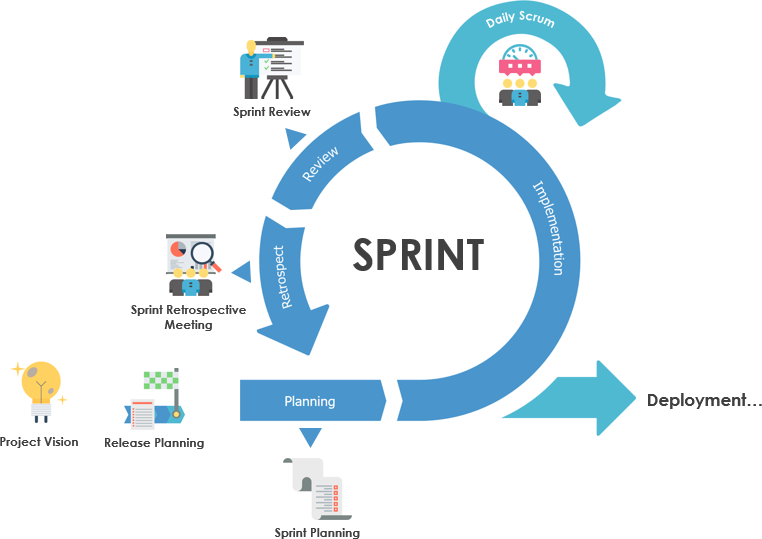
\includegraphics[width=7cm]{scrum}
		\caption{Metodo Scrum}
	\end{center}
\end{figure}
La situazione di emergenza sanitaria ancora non conclusa mi ha portato a vivere un'esperienza lavorativa diversa dai colleghi degli anni precedenti, infatti ha fatto sì che lo stage fosse organizzato in modalità mista: in parte da remoto ed in parte in azienda (di solito uno o due giorni alla settimana). A causa di ciò non ho potuto vivere appieno questo modello di sviluppo vista l'impossibilità di essere sempre presente in azienda. Per questo motivo il giorno concordato con i colleghi stagisti ed il tutor aziendale per andare in azienda è stato sfruttato per fare un daily scrum alternativo data la sua cadenza settimanale.\\ 
Nonostante l'emergenza sanitaria ancora in corso ho potuto comunque constatare l’efficacia e la funzionalità di questo modello di sviluppo, soprattutto per un progetto software in evoluzione quale è stato quello a cui ho lavorato.\\

\subsection{Organizzazione del lavoro}

\subsubsection{Trello}

Per tenere traccia delle attività da svolgere è stato deciso di utilizzare la piattaforma online Trello. Tramite essa l'azienda ha creato due bacheche:
\begin{itemize}
	\item personale: disponibile solo allo stagista ed al tutor aziendale, dove sono stati inseriti i compiti decisi nel piano di lavoro suddivisi per settimana;
	\item collettiva: disponibile a tutti gli stagisti che lavorano allo stesso progetto e ai loro rispettivi tutor aziendali, dove sono state inserite le prime idee e funzionalità legate al progetto.
\end{itemize}

\subsubsection{Report giornaliero}

Oltre a tenere traccia delle attività tramite Trello, l'azienda ha deciso di far scrivere allo stagista un file Excel su Drive come report giornaliero delle attività svolte. Il report era suddiviso in quattro colonne:
\begin{itemize}
	\item data: indica il giorno in è stata fatta un'attività in formato AAAA-MM-GG;
	\item descrizione: breve descrizione dell'attività svolta dal tirocinante compilata alla fine di ogni giornata lavorativa;
	\item nota: campo dove il tutor aziendale può aggiungere note di consiglio riguardo all'attività svolta, inoltre in questo campo vengono specificati i giorni festivi;
	\item spunta: casella di spunta dove il tutor indica di aver visionato l'attività svolta.
\end{itemize}

\begin{figure}[h]
	\begin{center}
		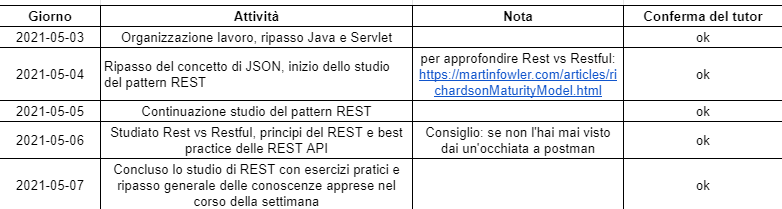
\includegraphics[width=14cm]{report}
		\caption{Spezzone del report giornaliero}
	\end{center}
\end{figure}

%**************************************************************

\subsubsection{Discord}

Per comunicare con l'intero gruppo di stagisti l'azienda ha proposto di utilizzare Discord, una piattaforma messaggistica dove noi stagisti potevamo comunicare sia con il personale aziendale che singolarmente con il proprio tutor per consigli, delucidazioni o motivi organizzativi.